\documentclass{article}
\usepackage{graphicx,fancyhdr,amsmath,amssymb,amsthm,subfig,url,hyperref}
\usepackage{enumitem}
\usepackage{tikz}
\usetikzlibrary{positioning, arrows.meta}
\usepackage[margin=1in]{geometry}

%----------------------- Macros and Definitions --------------------------

%%% FILL THIS OUT
\newcommand{\studentname}{Bhavya Patel}
\newcommand{\ruid}{bbp53}
\newcommand{\exerciseset}{Homework 1}
%%% END



%\renewcommand{\theenumi}{\bf \Alph{enumi}}

%\theoremstyle{plain}
%\newtheorem{theorem}{Theorem}
%\newtheorem{lemma}[theorem]{Lemma}

\fancypagestyle{plain}{}
\pagestyle{fancy}
\fancyhf{}
\fancyhead[RO,LE]{\sffamily\bfseries\large Rutgers University}
\fancyhead[LO,RE]{\sffamily\bfseries\large CS440 Intro to AI}
\fancyfoot[LO,RE]{\sffamily\bfseries \studentname (NetID: \ruid)}
\fancyfoot[RO,LE]{\sffamily\bfseries\thepage}
\renewcommand{\headrulewidth}{1pt}
\renewcommand{\footrulewidth}{1pt}

\graphicspath{{figures/}}

%-------------------------------- Title ----------------------------------

\title{CS440 \exerciseset}
\author{\studentname \quad (NetID: \ruid)\\ Number of late days I'd like to use is 0 (max 2):}

%--------------------------------- Text ----------------------------------

\begin{document}
\maketitle

\section*{Problem 1}
\begin{enumerate}[label=(\alph*)]
\item %A
State space A
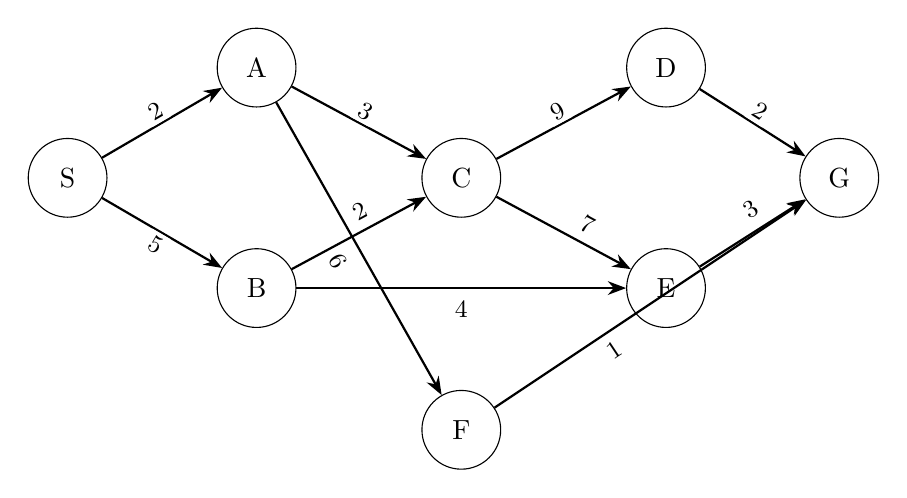
\begin{tikzpicture}[
  >=Stealth,
  edge/.style={->, thick},
  state/.style={circle, draw, minimum size=10mm, inner sep=0pt, font=\normalsize},
  wlabel/.style={midway, fill=white, inner sep=1.5pt, font=\small}
]

% --- Nodes ---
\node[state] (S) at (0,0) {S};

\node[state] (A) at (2.4, 1.4) {A};
\node[state] (B) at (2.4,-1.4) {B};

\node[state] (C) at (5.0, 0.0) {C};

\node[state] (D) at (7.6, 1.4) {D};
\node[state] (E) at (7.6,-1.4) {E};

\node[state] (F) at (5.0,-3.2) {F};
\node[state] (G) at (9.8, 0.0) {G};

% --- Edges ---
\draw[edge] (S) -- node[wlabel, sloped, above] {2} (A);
\draw[edge] (S) -- node[wlabel, sloped, below] {5} (B);

\draw[edge] (A) -- node[wlabel, sloped, above] {3} (C);

% A -> F label moved further away from the long diagonal
\draw[edge] (A) -- node[wlabel, sloped, below, yshift=-4pt] {6} (F);

% B -> C label moved slightly so it doesn't clash near C
\draw[edge] (B) -- node[wlabel, sloped, above, xshift=4pt, yshift=2pt] {2} (C);

% B -> E label stays centered but pushed down (avoids crowding near E)
\draw[edge] (B) -- node[wlabel, below, yshift=-3pt] {4} (E);

\draw[edge] (C) -- node[wlabel, sloped, above] {9} (D);

% C -> E label pushed right/up to avoid the E-node and other labels
\draw[edge] (C) -- node[wlabel, sloped, above, xshift=6pt, yshift=2pt] {7} (E);

% D -> G label fine
\draw[edge] (D) -- node[wlabel, sloped, above] {2} (G);

% E -> G label moved above and slightly right so it doesn't sit on the node/edge
\draw[edge] (E) -- node[wlabel, sloped, above, xshift=4pt, yshift=3pt] {3} (G);

% F -> E label moved closer to F side and below the edge to avoid E clutter
\draw[edge] (F) -- node[wlabel, sloped, below, pos=0.35, yshift=-2pt] {1} (G);

\end{tikzpicture}
\item % (b)
Using the given state-space graph (expanding neighbors in alphabetical order):

\textbf{BFS:} $S \rightarrow A \rightarrow F \rightarrow G$ \\
\textbf{BFS cost:} $2 + 6 + 1 = 9$ \\ 
\textbf{States Expanded:} $7$

\medskip

\textbf{DFS:} $S \rightarrow A \rightarrow C \rightarrow D \rightarrow G$ \\
\textbf{DFS cost:} $2 + 3 + 9 + 2 = 16$ \\ 
\textbf{States Expanded:} $4$

\medskip

\textbf{UCS:} $S \rightarrow A \rightarrow F \rightarrow G$ \\
\textbf{UCS cost:} $2 + 6 + 1 = 9$ \\
\textbf{States Expanded:} $6$

I think UCS finds the most optimal path ubt the costs of both BFS and UCS were the same but I think thats because its a small graph to work with \\ 
DFS finds it most quickly by expanding $4$ states. But it also has the most cost. It is unoptimal path that it yeidls

\item %C

Using the given heuristic values (and $h(G)=0$), expanding neighbors in alphabetical order:

\textbf{Greedy:} $S \rightarrow A \rightarrow C \rightarrow E \rightarrow G$ \\
\textbf{Greedy cost:} $2+3+7+3=15$ \\
\textbf{States Expanded:} 4

\medskip
\textbf{A*:} $S \rightarrow B \rightarrow E \rightarrow G$ \\
\textbf{A* cost:} $5+4+3=12$ \\
\textbf{States Expanded:} 5

\medskip
\textbf{Optimal from (b):} $S \rightarrow A \rightarrow F \rightarrow G$ \\
\textbf{Optimal cost:} $2+6+1=9$

\medskip
Greedy and A* both differ from the optimal path because this heuristic is \textbf{not admissible}
(e.g., $h(F)=5 > 1$ and $h(D)=3 > 2$) and \textbf{not consistent}
(e.g., $h(F) \nleq 1+h(G)$), so Greedy can be misled and A* is not guaranteed to return the opti*


\end{enumerate}

\section*{Problem 2}
\begin{enumerate}[label=(\alph*)]

\item % (a)
Let the state be $(x,v)$ and action $a\in\{-1,0,+1\}$. The intended next velocity is $v' = v+a$
and the next position is $x' = x+v'$.

\medskip
\noindent If $a\in\{0,+1\}$ (no braking involved):
\[
T\big((x+v+a,\; v+a)\mid (x,v), a\big)=1.
\]

\medskip
\noindent If $a=-1$ (brake failure w.p. $\alpha$):
\[
T\big((x+v-1,\; v-1)\mid (x,v),-1\big)=1-\alpha,
\qquad
T\big((x+v,\; v)\mid (x,v),-1\big)=\alpha.
\]

\item % (b)
Given $\gamma=1$, no speed bumps, and terminal reward $R$ at the school:

\medskip
\noindent \textbf{$\pi_1$:} always keep speed $v=1$ \\
\textbf{$\pi_1$ return:} $U(\pi_1)=R-4$ \\
For $R=15$: $U(\pi_1)=11$

\medskip
\noindent \textbf{$\pi_2$:} speed up to $v=2$, then brake once near the end \\
\textbf{$\pi_2$ return:} 
\[
U(\pi_2)=(-1)+(-1)+(1-\alpha)(R-1)+\alpha(-1)=(1-\alpha)R-3
\]
For $\alpha=0.1,\ R=15$: $U(\pi_2)=10.5$

\medskip
\noindent \textbf{Comparison:} $U(\pi_1)=11 > U(\pi_2)=10.5$, so $\pi_1$ is better here. \\
\textbf{When is $\pi_2$ better?}
\[
(1-\alpha)R-3 > R-4 \;\Longleftrightarrow\; \alpha R < 1.
\]

\item % (c)
Now $n=11$, speed bump at $x=5$ with speed limit $k=1$, $m=3$, $\alpha=0.1$, $R=15$, $\gamma=1$.
If the car enters/passes the bump or enters the school with $v>1$, the terminal reward becomes $0$.

\medskip
\noindent \textbf{$\pi_1$:} safely keep $v=1$ the whole way to the school \\
\textbf{$\pi_1$ return:} $V^{\pi_1}(1,0)=(R-1)-9=14-9=5$

\medskip
\noindent \textbf{Improved $\pi_2$:} go $v=1$ through the bump, then speed up after the bump and brake early enough to retry if braking fails \\
\textbf{$\pi_2$ return (from code):} $V^{\pi_2}(1,0)=5.95$

\medskip
\noindent \textbf{Conclusion:} $\pi_2$ is better than $\pi_1$ here since $5.95 > 5$.

\end{enumerate}

\section*{Problem 3}
\begin{enumerate}[label=(\alph*)]

\item % (a)
We are asked for $V_{\text{walk}}(s)$ and $V_{\text{bus}}(s)$ for the two fixed policies (with $\gamma=1$). 
The reward definitions imply walking costs $1$ unit of time per step (reward $=-1$), and the bus costs
$1+\alpha(n-s)$ time if it arrives (reward $=-1-\alpha(n-s)$) and costs $1$ time if it does not arrive (reward $=-1$). :contentReference[oaicite:2]{index=2}

\medskip
\noindent \textbf{Always Walk:} each step moves from $s$ to $s+1$ with reward $-1$. To reach $n$ takes $(n-s)$ steps.
\[
V_{\text{walk}}(s)=-(n-s).
\]

\medskip
\noindent \textbf{Always Bus:} each attempt takes 1 time unit. With probability $\epsilon$ the bus arrives and you go to $n$
(with extra time $\alpha(n-s)$), and with probability $1-\epsilon$ you stay at $s$.
The expected number of attempts until success is $1/\epsilon$. Therefore expected time is
\[
\mathbb{E}[T] = \frac{1}{\epsilon} + \alpha(n-s),
\]
so the expected reward (negative time) is
\[
V_{\text{bus}}(s)= -\left(\frac{1}{\epsilon}+\alpha(n-s)\right)= -\frac{1}{\epsilon}-\alpha(n-s).
\]

\item % (b)
Run one pass of Q-learning over the provided data (left-to-right) with $\eta=0.5$, $\gamma=1$, and all $\hat Q=0$ initially.

\medskip
\noindent \textbf{Update rule:}
\[
\hat Q(s,a)\leftarrow \hat Q(s,a)+\eta\Big(r+\gamma\max_{a'}\hat Q(s',a')-\hat Q(s,a)\Big).
\]

\medskip
\noindent \textbf{Step 1: } $(1,\text{Bus},-1,1)$
\[
\hat Q(1,\text{Bus}) = 0 + 0.5(-1+0-0) = -0.5.
\]

\medskip
\noindent \textbf{Step 2: } $(1,\text{Bus},-1,1)$
\[
\max_{a'}\hat Q(1,a')=\max(-0.5,0)=0
\]
\[
\hat Q(1,\text{Bus}) = -0.5 + 0.5(-1+0-(-0.5)) = -0.75.
\]

\medskip
\noindent \textbf{Step 3: } $(1,\text{Bus},3,3)$
\[
\max_{a'}\hat Q(3,a')=0
\qquad\Rightarrow\qquad
\hat Q(1,\text{Bus}) = -0.75 + 0.5(3-(-0.75)) = 1.125.
\]

\medskip
\noindent \textbf{Step 4: } $(3,\text{Walk},1,4)$
\[
\max_{a'}\hat Q(4,a')=0
\qquad\Rightarrow\qquad
\hat Q(3,\text{Walk}) = 0 + 0.5(1)=0.5.
\]

\medskip
\noindent \textbf{Step 5: } $(4,\text{Walk},1,5)$
\[
\max_{a'}\hat Q(5,a')=0
\qquad\Rightarrow\qquad
\hat Q(4,\text{Walk}) = 0 + 0.5(1)=0.5.
\]

\medskip
\noindent \textbf{Final requested values (from the above pass):} \\
$\hat Q(1,\text{Bus})$ after step 1: $-0.5$ \\
$\hat Q(1,\text{Bus})$ after full pass: $1.125$ \\
$\hat Q(3,\text{Walk})$: $0.5$ \\
$\hat Q(4,\text{Walk})$: $0.5$


\item % (c)
Christopher takes the bus when $s<\tfrac{3}{4}n$ and walks when $s\ge \tfrac{3}{4}n$. :contentReference[oaicite:4]{index=4}

\medskip
\noindent (i) A clean policy function:
\[
\pi(s)=
\begin{cases}
\text{Bus} & \text{if } s < \tfrac{3}{4}n\\
\text{Walk} & \text{if } s \ge \tfrac{3}{4}n
\end{cases}
\]

\medskip
\noindent (ii) I would \textbf{not} suggest Q-learning if the goal is just the expected commute time under this fixed policy.
Q-learning targets the \emph{optimal} $Q^*$, while here we just want to evaluate $V^\pi$ (policy evaluation).
A simpler approach is Monte Carlo (average episode returns) or TD(0) value estimation following $\pi$.

\item % (d)
Christopher uses TD-learning while following $\pi$ from (c) to estimate $V^\pi(s)$. :contentReference[oaicite:5]{index=5}

\medskip
\noindent (i) Not necessarily. A potential convergence issue is \textbf{lack of coverage}: under the policy in (c),
some states may be visited very rarely (or effectively never) because taking the bus can jump directly to $n$,
so TD updates for those states do not happen enough to converge.

\medskip
\noindent (ii) Modify to a policy $\pi'$ that guarantees exploration/visitation across all states, e.g.
an $\epsilon$-soft version of $\pi$:
with probability $(1-\epsilon)$ take $\pi(s)$, and with probability $\epsilon$ take the other action.
This way every state-action can be sampled and TD estimates stabilize.

\item % (e)
To collect more data while still getting to the gym reasonably quickly and ensuring convergence,
use an \textbf{$\epsilon$-greedy (or generally $\epsilon$-soft / GLIE)} exploration policy:
mostly choose the currently best action, but sometimes explore the other action so that all states keep getting updated.

\end{enumerate}



\end{document}
